% !TeX encoding = UTF-8

\documentclass{LTHtwocol} % Use this when you work on your report.
% \documentclass[final]{LTHtwocol} % Use this for the final version.
                                   % It will remove page numbers and
                                   % markers for overfull boxes.
                                   % There really shouldn't be any of those anyway.

\usepackage[utf8]{inputenc}        
\usepackage{amsmath,amssymb,graphicx}

\usepackage{xcolor}
\usepackage{hyperref} 
\hypersetup{
	colorlinks,
	linkcolor={red!50!black},
	citecolor={blue!50!black},
	urlcolor={blue!80!black}
}

\usepackage{kantlipsum} % Only for the dummy text. Remove for your own report.

\addbibresource{bibliography.bib}

% Document begins here
\begin{document}
\begin{frontmatter}
\title{Project Title} % Title of the project.
                      % Note that all reports are in English,
                      %so that our international students can read them.

\author[anna]{Anna Andrén}
\author[bertil]{Bertil Bengtsson}
\author[cecilia]{Cecilia Clarin}
\author[david]{David Delin}

\email[anna]{anna.andren@student.lth.se}
\email[bertil]{bertil.bengtsson@student.lth.se}
\email[cecilia]{cecilia.clarin@student.lth.se}
\email[david]{david.delin@student.lth.se}

\begin{abstract}
    The abstract should be a 200--250 word compact description of your project. What was the objective? Which methods did you use? What was the (main) result?
\end{abstract}

\end{frontmatter}

% Stick to the proposed structure below. Add \subsections{} as appropriate.
% This file compiles on the Automatic Control Department system by typing the
% following into the terminal (while in the directory of the file, and with all
% other files belonging to the template untouched):
% > pdflatex template        
% > biber template
% The first line compiles the .tex file. The second line generates the
% bibliography. Once this is done, you may need to run the first line 1-2
% additional times, for the system to get all cross references right in the
% produced pdf output.

\section{Introduction}
Here you introduce the project. What is the background? What project do you aim at solve? References to prior work? If the project makes a positive or negative environmental, or other solitary, impact, describe it here. Are there any ethical considerations? You might want to reference relevant literature, e.g. \cite{openclosed2, Hellerstein2004, Yun2015}. A general \LaTeX\ guide is available at \cite{latexwiki}. 

\subsection{Some Dummy Text}
\kant[1] % This generates the dummy text

\section{Modeling}
Here you present the modeling approach and publish your model. If your model has 63434 parameters, you may not wish to print it in detail. The idea is, however, that another group with your background should be able to reproduce your work -- this goes not only for the modeling aspect.

If you use equations, make sure they are all numbered:
\begin{equation}
\alpha_a^2 + \beta_b^2 = \gamma_c^2.
\label{eq:formula}
\end{equation}
Equations are parts of the text. If they end a sentence, they should end with a dot. If they end a clause, they should end with a comma. You refer to an equation this like: see \eqref{eq:formula}. Note that all units are written in roman type: $\omega=2\pi$~rad/s, $g = 9.81$~m/s$^2$. See \cite{mathslatexwiki} for a tutorial on typesetting maths.

\subsection{Some Dummy Text}
\kant[2]

\section{System Design}
Describe the control or learning system you have designed.
Did you build anything? If so, what did you build, and using what production methods. If you built the hardware or were handed it, \emph{a photograph of your gadget is mandatory}. Make sure any figures are referenced from from the text---like this, see Figure~\ref{fig:gadget}---and that they all have a descriptive caption.
\begin{figure}[b]
	\centering
	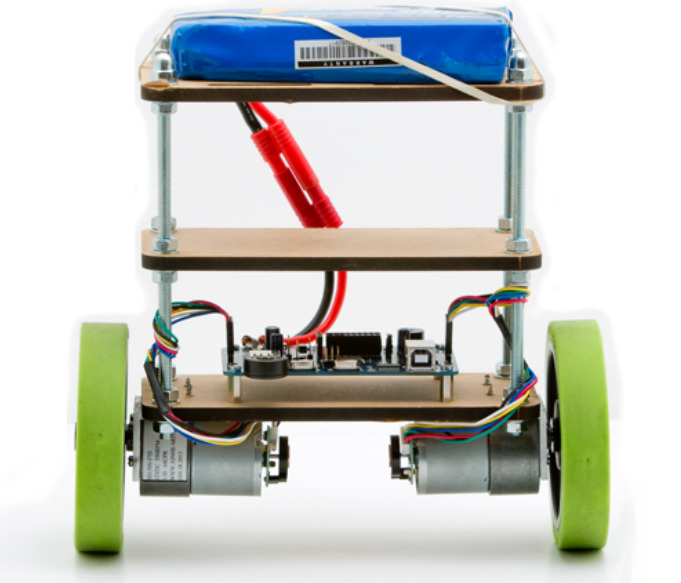
\includegraphics[width=0.7\columnwidth]{balanduino}
	\caption{Example picture of the Balanduino robot. Place all figures at the top \texttt{[t]} (default) or bottom \texttt{[b]} (only if needed).}
	\label{fig:gadget} % Should be placed after the caption!
\end{figure}

\subsection{Some Dummy Text}
\kant[3]

\section{Implementation}
Here you describe how you implemented your learning or control design. 

\section{Results}
If you need to use tables, Table~\ref{tab:extable} shows an example of how they can be typeset. For further details, see \cite{tablelatexwiki}.

\begin{table}[t]
	\centering
	\caption{Example table. Note that the caption goes on top. Place all tables at the top \texttt{[t]} (default) or bottom \texttt{[b]} (only if needed) of the page.}
	\label{tab:extable}
	\begin{tabular}{lcrrcrrcrr} % (l)eft, (r)ight and (c)enter indentation
		\toprule
        & 
		\multicolumn{2}{c}{IAE [$\cdot 10^3$~s]} & &
		\multicolumn{2}{c}{$\text{var}(\tau^o)$ [s]} & &  
		\multicolumn{2}{c}{$\tau^o_{max}$ [s]} \\[1mm]
		$M_C$            &  3     & 10  &~& 3     & 10    &~& 3    & 10 \\ 
        \midrule
		$C_{\text{orig}}$ & 8.23 & 8.34 &~& 0.695 & 0.745 &~& 5.68 & 6.27 \\ 
		$C_{\text{fb}}$ & 1.48 & 0.98 &~& 0.030 & 0.021 &~& 1.81 & 1.83 \\ 
		$C_{\text{ff}}$ & 1.23 & 1.43 &~& 0.026 & 0.034 &~& 1.56 & 1.65\\
        \bottomrule 
	\end{tabular}
\end{table}

\subsection{Some Dummy Text}
\kant[4]

\section{Discussion}

Discuss the results and what you learned from the project.


% Prints cited references
\printbibliography


\end{document}


